\section{Muhammad Reza Syachrani - 1174084}
\subsection{Teori}
\begin{enumerate}

	\item Jelaskan dengan ilustrasi gambar sendiri apa perbedaan antara vanilla GAN dan cGAN
	\hfill\\
Vanilla GAN adalah tipe GAN paling sederhana. Di sini, Generator dan Diskriminator adalah perceptron multi-layer sederhana. sedangkan  pada CGAN (Conditional GAN)  parameter ditambahkan ‘y’ ke Generator untuk menghasilkan data yang sesuai. Label juga dimasukkan ke dalam input ke Diskriminator agar Diskriminator membantu membedakan data nyata dari data yang dihasilkan palsu.
Untuk ilustrasi, lihat gambar berikut:

\begin{figure}[H]
    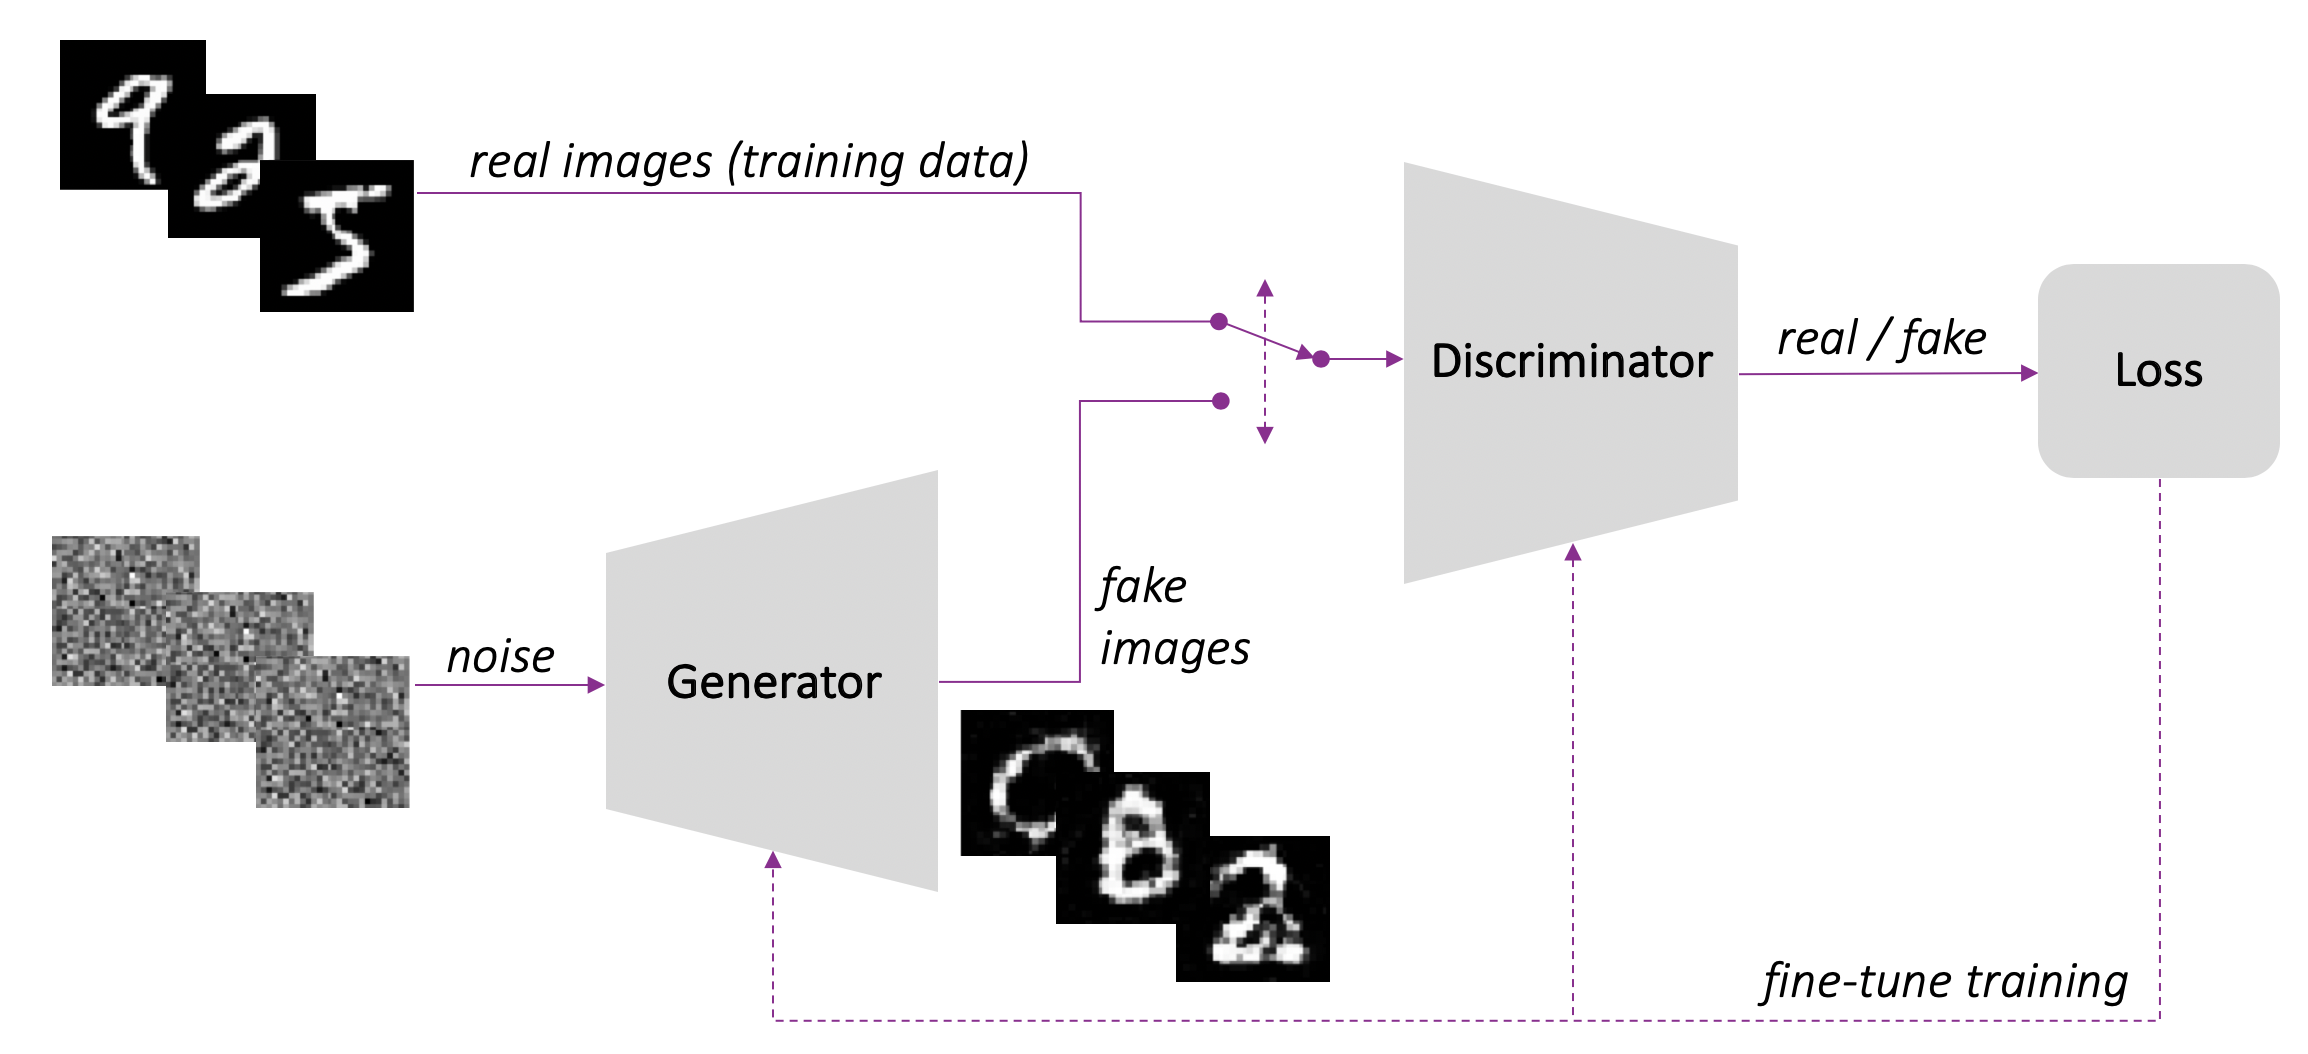
\includegraphics[width=12cm]{figures/1174084/9/teori1.png}
    \centering
    \caption{Teori 1}
\end{figure}
\begin{figure}[H]
    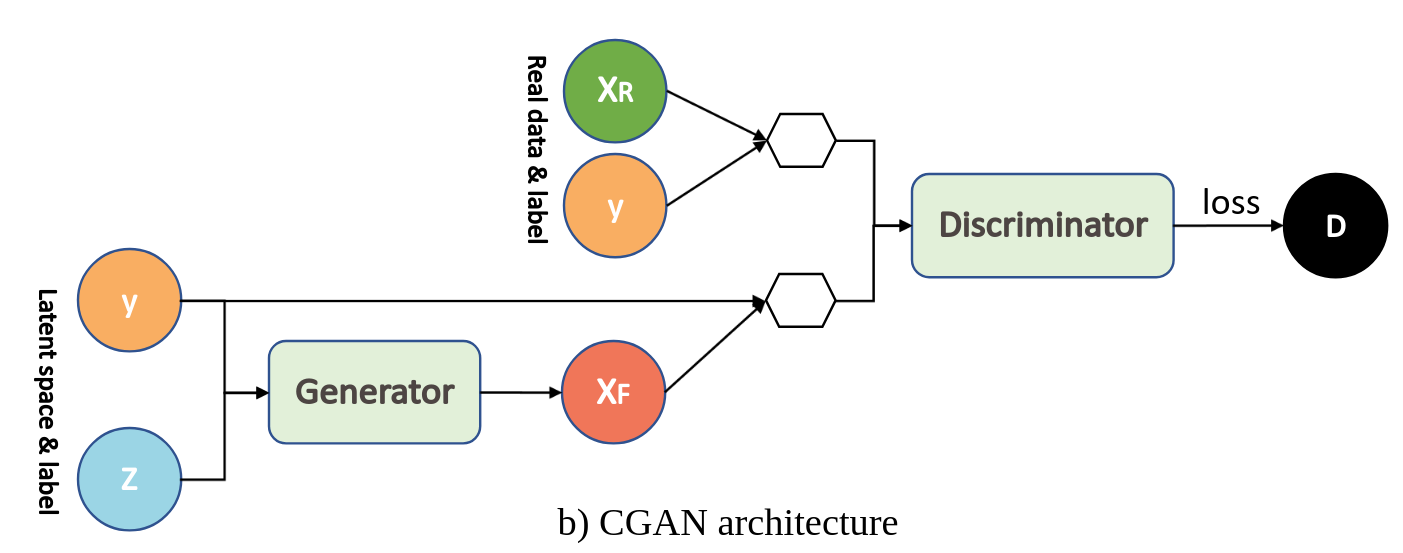
\includegraphics[width=12cm]{figures/1174084/9/teori1_1.png}
    \centering
    \caption{Teori 1}
\end{figure}

\item Jelaskan dengan ilustrasi gambar sendiri arsitektur dari Age-cGAN.
	\hfill\\
	 Age-cGan terdiri dari empat jaringan: encoder, FaceNet, jaringan generator, dan jaringan diskriminator 
	Untuk ilustrasi, lihat gambar berikut:  

\begin{figure}[H]
    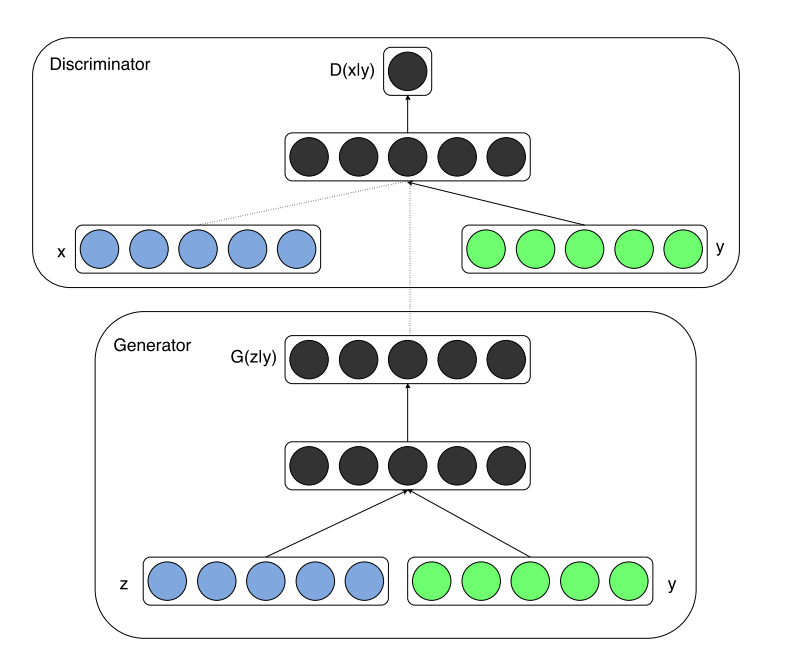
\includegraphics[width=12cm]{figures/1174084/9/teori2.png}
    \centering
    \caption{Teori 2}
\end{figure}

\item Jelaskan dengan ilustrasi gambar sendiri arsitektur encoder network dari AgecGAN
	\hfill\\
	 jaringan encoder adalah untuk menghasilkan vektor laten dari gambar yang disediakan. Pada dasarnya, ini mengambil gambar dari dimensi (64, 64, 3) dan mengubahnya menjadi vektor 100 dimensi. Jaringan encoder adalah jaringan saraf convolutional yang mendalam.
	
	Untuk ilustrasi, lihat gambar berikut:

\begin{figure}[H]
    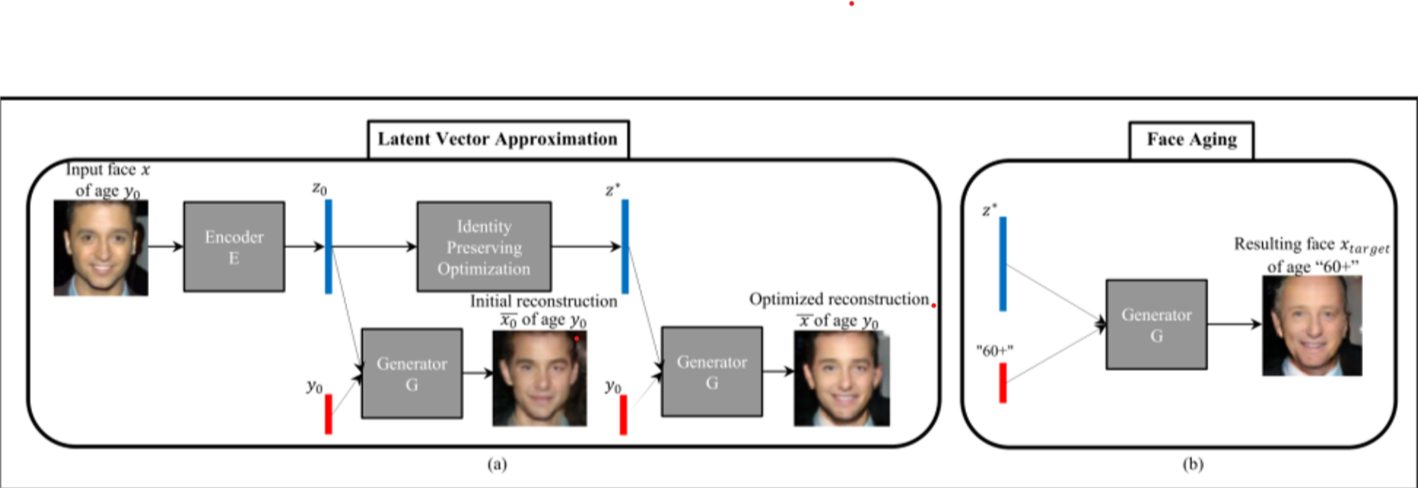
\includegraphics[width=12cm]{figures/1174084/9/teori345.png}
    \centering
    \caption{Teori 3}
\end{figure}

\item Jelaskan dengan ilustrasi gambar sendiri arsitektur generator network dari AgecGAN.
\hfill\\
	 jaringan generator adalah untuk menghasilkan gambar dengan dimensi (64, 64, 3). Dibutuhkan vektor laten 100 dimensi dan beberapa informasi tambahan, y, dan mencoba menghasilkan gambar yang realistis.
	
	
\begin{figure}[H]
    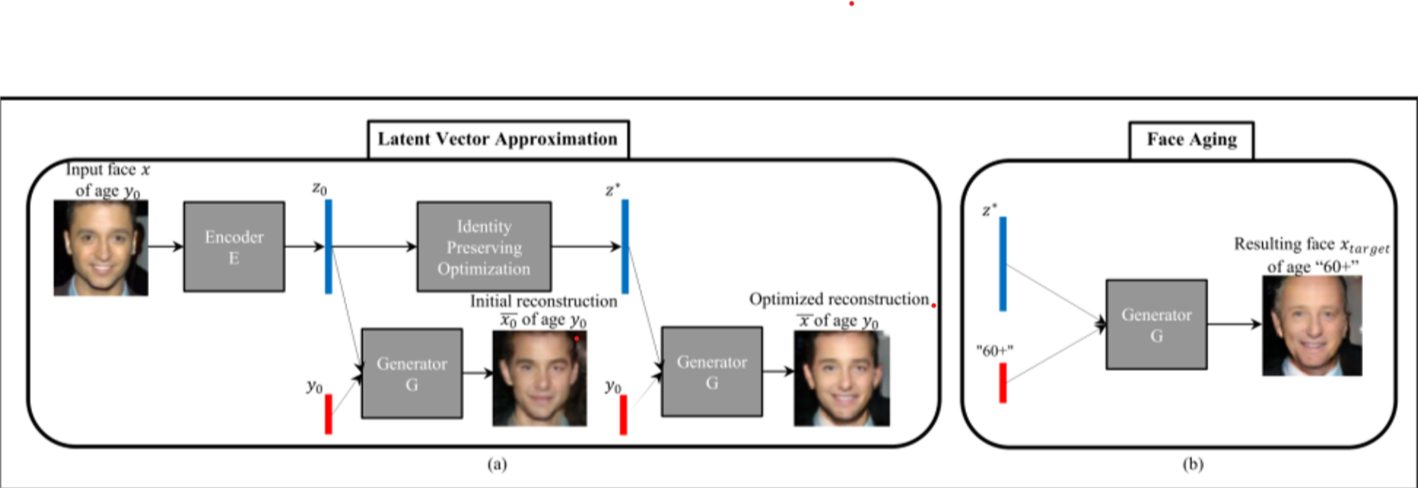
\includegraphics[width=8cm]{figures/1174084/9/teori345.png}
    \centering
    \caption{Teori 4}
\end{figure}

\item Jelaskan dengan ilustrasi gambar sendiri arsitektur discriminator network dari Age-cGAN
	\hfill\\
	jaringan diskriminator adalah untuk mengidentifikasi apakah gambar yang disediakan adalah palsu atau nyata. Ini dilakukan dengan melewatkan gambar melalui serangkaian lapisan downsampling dan beberapa lapisan klasifikasi.
	ilustrasi pada gambar berikut :

\begin{figure}[H]
    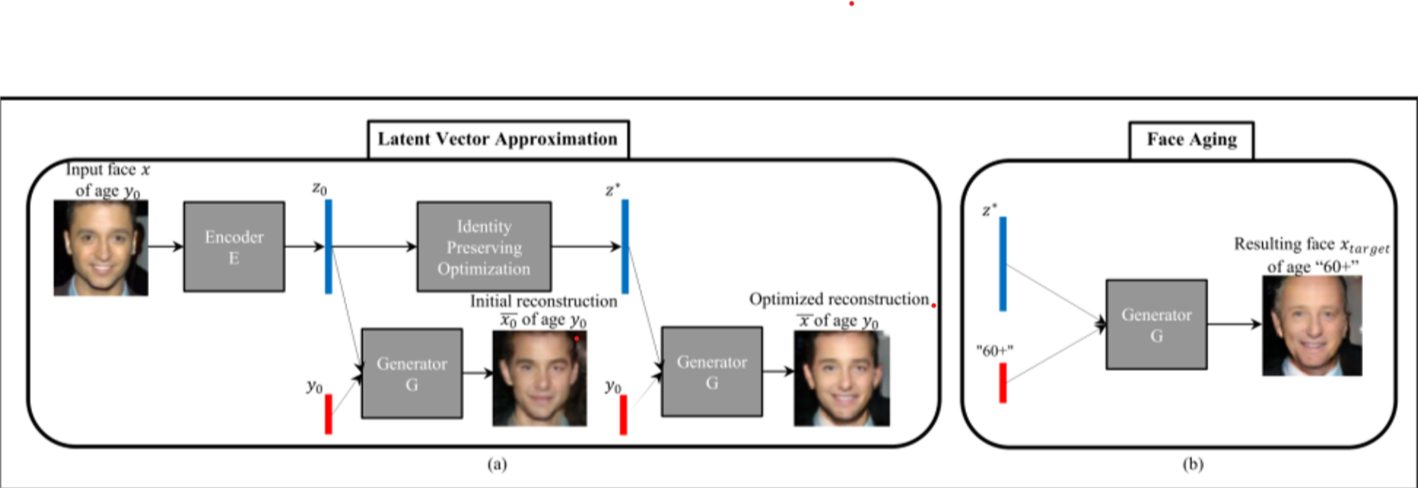
\includegraphics[width=8cm]{figures/1174084/9/teori345.png}
    \centering
    \caption{Teori 5}
\end{figure}

\item Jelaskan dengan ilustrasi gambar apa itu pretrained Inception-ResNet-2 Model
	\hfill\\
	Pre-Trained Network atau Transfer Learning merupakan suatu metode penyelesaian yang memanfaatkan model yang sudah dilatih terhadap suatu dataset untuk menyelesaikan masalah dengan cara menggunakan sebagai starting point, memodifikasi dan mengupdate parameternya, sehingga sesuai dengan dataset yang baru.
	
	
\begin{figure}[H]
    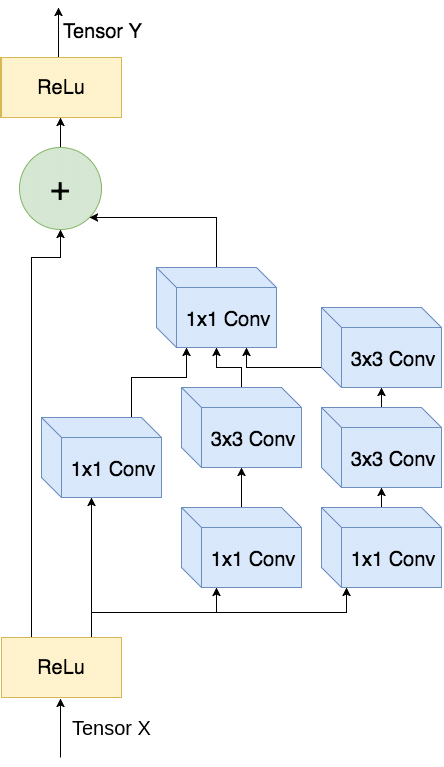
\includegraphics[width=8cm]{figures/1174084/9/teori6.png}
    \centering
    \caption{Teori 6}
\end{figure}

\item Jelaskan dengan ilustrasi gambar sendiri arsitektur Face recognition network Age-cGAN
	\hfill\\
	Face recognition network Age-cGAN adalah untuk mengenali identitas seseorang dalam gambar yang diberikan. dengan mempelajari perbedaan antara gambar input x dan gambar yang direkonstruksi
		
\begin{figure}[H]
    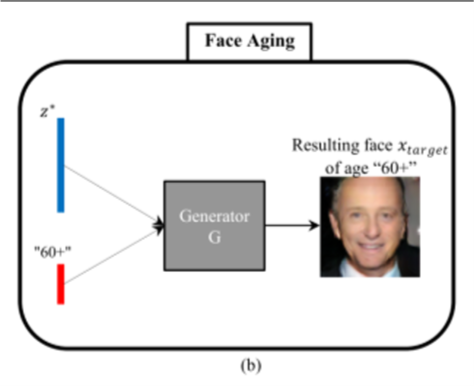
\includegraphics[width=8cm]{figures/1174084/9/teori7.png}
    \centering
    \caption{Teori 7}
\end{figure}

\item Sebutkan dan jelaskan serta di sertai contoh-contoh tahapan dari Age-cGA
	\hfill\\
	Pelatihan Age-cGAN terdiri dari tiga tahap: 
	\begin{enumerate}
	\item Conditional GAN training: Pada tahap ini, kami melatih jaringan generator dan jaringan diskriminator.
	\item Initial latent vector approximation : Pada tahap ini, kami melatih jaringan pembuat enkode.
	\item Latent vector optimization: Pada tahap ini, kami mengoptimalkan encoder dan jaringan generator.
	\end{enumerate}
	
	
\item Berikan contoh perhitungan fungsi training objektif
	\hfill\\
	Objektif Trainning ialah untuk meminimalkan loss function sebagai log likelihood function yang diberikan pada persamaan dimana D melambangkan trainning data.
	
\begin{figure}[H]
    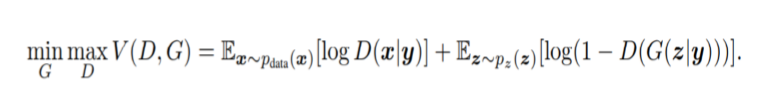
\includegraphics[width=8cm]{figures/1174084/9/teori9.png}
    \centering
    \caption{Teori 9}
\end{figure}


\item Berikan contoh dengan ilustrasi penjelasan dari Initial latent vector approximation
	\hfill\\
	Latent vector approdimation kemampuan untuk membuat gambar yang realistis dan tajam serta menghasilkan gambar wajah pada usia target.
			
	

\item Berikan contoh perhitungan latent vector optimization
	\hfill\\
	Perhitungan latent optimization menggunakan metode yang relatif sederhana, tergantung pada jumlah kecil parameter yang diperlukan, sehingga pada latent optimization dapat memetakan setiap gambar x dari dataset ke vektor acak dimensi rendah zi dalam ruang laten z.	
	
\begin{figure}[H]
    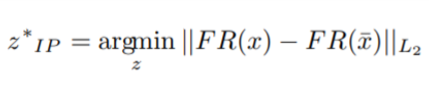
\includegraphics[width=8cm]{figures/1174084/9/teori11.png}
    \centering
    \caption{Teori 11}
\end{figure}	
	
\end{enumerate}


\subsection{Praktek}
\begin{enumerate}

\item Jelaskan bagaimana cara ekstrak file dataset Age-cGAN menggunakan google colab.
	\hfill\\
	\begin{itemize}
		\item Login ke google colab menggunakan akun google
		\item Mount google drive
		\item Lakukan proses unzip melalui notebook python di google colab, unzip pakai codingan
		\item Selesai
	\end{itemize}
		\lstinputlisting[firstline=13, lastline=15]{src/1174084/9/1174084.py}

	\item Jelaskan bagaimana kode program bekerja untuk melakukan load terhadap dataset yang sudah di ekstrak, termasuk bagaimana penjelasan kode program perhitungan usia.
	\hfill\\
	Dibawah ini merupakan code untuk melakukan fungsi perhitungan usia.
		\lstinputlisting[firstline=209, lastline=233]{src/1174084/9/1174084.py}

	\item Jelaskan bagaimana kode program The Encoder Network bekerja dijelaskan dengan bahawa awam dengan ilustrasi sederhana.
	\hfill\\
	Proses Encoder berfungsi untuk mempelajari pemetaan terbalik dari gambar wajah dan kondisi usia dengan vector latent Z.
		\lstinputlisting[firstline=40, lastline=79]{src/1174084/9/1174084.py}

	\item Jelaskan bagaimana kode program The Generator Network bekerja  dengan ilustrasi sederhana.
	\hfill\\
	Proses Generator agar bekerja dengan baik dibutuhkan representasi dari gambar wajah dan vector kondisi sebagai inputan yang menghasilkan sebuah gambar.
		\lstinputlisting[firstline=81, lastline=119]{src/1174084/9/1174084.py}

	\item Jelaskan bagaimana kode program The Discriminator Network bekerja dijelaskan dengan bahawa awam dengan ilustrasi sederhana.
	\hfill\\
	Proses Discriminator untuk membedakan antara gambar asli dan gambar palsu.
		\lstinputlisting[firstline=127, lastline=158]{src/1174084/9/1174084.py}

	\item Jelaskan bagaimana kode program Training cGAN bekerja dijelaskan dengan bahawa awam dengan ilustrasi sederhana.
	\hfill\\
	Proses Training cGAN ini dengan load file .mat pada dataset lalu epoch sebanuak 500 kali.
		\lstinputlisting[firstline=312, lastline=328]{src/1174084/9/1174084.py}

	\item Jelaskan bagaimana kode program Initial dan latent vector approximation bekerja dijelaskan dengan bahawa awam dengan ilustrasi sederhana.
	\hfill\\
	Initial dan Latent Vector Approximation bekerja melakukan prediksi epoch yang telah di buat sebanyak 500 kali, dan hasilnya disimpan pada folder result.
		\lstinputlisting[firstline=450, lastline=493]{src/1174084/9/1174084.py}
		
\end{enumerate}


\subsection{Bukti Tidak Plagiat}
\begin{figure}[H]
	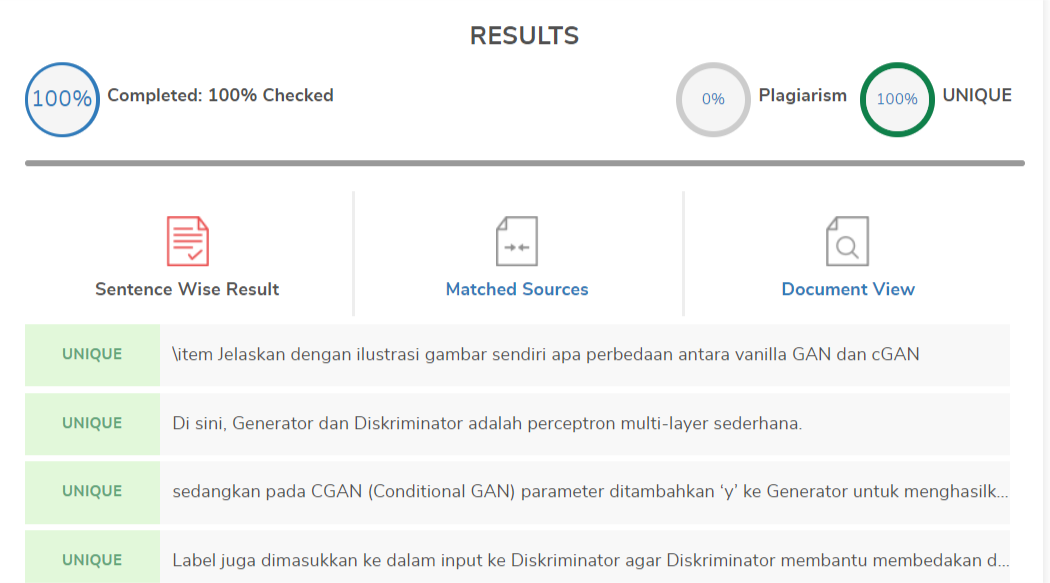
\includegraphics[width=4cm]{figures/1174084/9/plagiarism.png}
	\centering
	\caption{plagiarism}
\end{figure}


\subsection{Link Video Youtube}
https://youtu.be/fnc2PcVDkOU

